\documentclass[12pt]{report}
% \usepackage{minted}
\usepackage{xcolor}
\definecolor{light-gray}{rgb}{0.9,0.9,0.9}
% \usepackage{emptypage}
\usepackage[T1]{fontenc}
\usepackage{textcomp}
\usepackage[utf8]{inputenc}
% \usepackage[italian]{babel}
\usepackage{graphicx}
\graphicspath{ {Images/} }
\usepackage{caption}
\usepackage{subcaption}
\usepackage{enumerate}
\usepackage{array}
\usepackage{tabularx}
\usepackage{float}
\usepackage[a4paper,width=150mm,top=30mm,bottom=30mm,left=30mm,right=30mm,bindingoffset=6mm]{geometry}
\usepackage{fancyhdr}
\linespread{1.3}\selectfont

\usepackage{titlesec}
\titleformat{\chapter}{}{}{0em}{\bf\LARGE}

\usepackage{hyperref}
\hypersetup{
    colorlinks,
    citecolor=black,
    filecolor=black,
    linkcolor=black,
    urlcolor=black
}


\begin{document}
    
  % TODO: Fill title page
  \begin{titlepage}
    
  \end{titlepage}
  
  \tableofcontents
   
  \chapter{Introduction}
  \section{Purpose}
  The purpose of this Requirement Analysis and Specification Document (RASD)
is to provide a detailed description about SafeStreets.
In particular, this document is focused on important aspects that are
useful during the design of the software architecture like: scope, functional and
non-functional requirements, use cases and scenarios, constraints and assumption, UML diagrams, limitation and interfaces with other software.
Overall the document is a useful guide for the developers that will have to follow
and implement all the necessary requirements; nevertheless it is also a document
that can be given to potential customers to get them an idea of what the software
will be like.\newline
The software features have been identified in the following list of goals.

\subsection{Goals}
\begin{itemize}
  \item {[G1]}: Allow a person to become a registered User after submitting his credentials for the registration to the service
  \item {[G2]}: Allow the user to send a violation report consisting in a picture and some metadata
    \begin{itemize}
      \item {[G2.1]}: Allow the user to send along with the picture the plate number
    \end{itemize}
  \item {[G3]}: Allow the user to watch the history of his reports and their status
  \item {[G4]}: Allow the user to watch on a map areas and streets with an high frequency of violations
  \begin{itemize}
    \item {[G4.1]}: The user gets the latest violations near its current location 
    \item {[G4.2]}: The user gets the latest violations near the location that he specifies
  \end{itemize} 
  \item {[G.5]}: Allow the local system administrator of the police station to create accounts for the police technician by giving him an administrator account
  \item {[G.6]}: Allow the authorities to visualize the reports submitted by the users
  \item {[G.7]}: Allow the authorities to mine the data to make analisys and retrieve statistics
  \item {[G.8]}: If the municipality offers a service that provides data about accidents then the system must be able to cross this data with its own data in order to identify possible unsafe areas
  \begin{itemize}
    \item {[G.8.1]}: In this case the system must be able to suggest possible interventions
    \item {[G.8.2]}: The users must be able  watch this unsafe areas
    \item {[G.8.3]}: The authorities must be able to consult the crossed data
  \end{itemize} 
\end{itemize}


  \section{Scope}
  % TODO: check the scope
Here is a brief review of what has already been said into the RASD document about the SafeStreet scope and functionalities.
\newline
SafeStreets is a new service that aims, via the help of citizens, to improve the safety of the streets. Users will have the possibility to send reports of illegal behaviour related to street parking to authorities, just by opening the safe SafeStreets mobile application and take a picture of the violation. Moreover they can also consult the history of their reports and a map that will highlight the most dangerous streets nearby. SafeStreets also offers a way for the authorities to manage the reports and perform analysis on the data. A Web interface will be developed in order to address this purpose. In order to guarantee and efficient use of the application by authorities, the system interacts with an external plate recognition service that will extract the car plate number from the report image. In this way when authorities need to check on a report they immediately find the car plate number of the vehicle that committed the violation. SafeStreets also implements a functionality that performs the interaction with a municipality service that offers data regarding car accidents, if the particular municipality offers one. SafeStreets can cross this information with its owns, in order to get a better idea of the potentially unsafe areas and therefore suggest some possible interventions.
As for the performances, the service will have to be scalable,
fast and it must be able to cover a great number of users. While for the applications they must be lightweight and must run of most of the devices available on the market.

  \section{Definitions, acronyms and abbreviations}
  \subsection{Definitions}
\begin{itemize}
  \item \textit{Most Dangerous Streets}: Streets with the highest frequency of violation reports.
\end{itemize}

\subsection{Acronyms}
\begin{itemize}
  \item EU: European Union;
  \item CET: Central European Timezone;
  \item API: Application Programming Interface;
  \item HTTP: Hyper Text Transfer Protocol;
  \item GPS: Global Positioning System;
  \item GDPR: General Data Protection Regulation;
  \item REST: Representational State Transfer.
  \item URL: Uniform resource locator
  \item URI: Uniform resource indicator
  \item DB: Database
  \item DBMS: Database management system
  \item RDBMS: Relational database management system
  \item SQL: Structured query language
  \item NoSQL: Not only SQL
\end{itemize}

\subsection{Abbreviations}
\begin{itemize}
  \item {[Gn]}: n-th goal;
  \item {[Dn]}: n-th domain assumption;
  \item {[Rn]}: n-th functional requirements;
  \item MDS: Most Dangerous Street;
  \item LSA: Local System Administrator;
  \item PT: Police Technician.
\end{itemize}

  \section{References}
  \begin{itemize}
    \item LateX Workshop extension for Visual Studio Code: \newline\href{https://github.com/James-Yu/LaTeX-Workshop/}{https://github.com/James-Yu/LaTeX-Workshop/}
    \item LateX compiler: \newline\href{https://www.latex-project.org/}{https://www.latex-project.org/}
    \item StarUML for UML diagrams:\newline\href{http://staruml.io/}{http://staruml.io/}
    \item DrawIO for some UML diagrams\newline\href{http://draw.io}{http://draw.io}
    \item MVC design pattern wikipedia: \newline\href{https://en.wikipedia.org/wiki/Model-view-controller}{https://en.wikipedia.org/wiki/Model-view-controller}
    \item Multitier architecture wikipedia: \newline\href{https://en.wikipedia.org/wiki/Multitier_architecture}{wikipedia}
    \item Relational database advantages: \newline\href{https://searchdatamanagement.techtarget.com/definition/relational-database}{https://searchdatamanagement.techtarget.com/definition/relational-database}
\end{itemize}
  \section{Revision History}
  \begin{itemize}
    \item Version 1:
        \begin{itemize}
            \item 1.0: First release.
            \item 1.1: Minor fixes to sequence diagrams
        \end{itemize}
\end{itemize}

  \section{Document Structure}
  % TODO: check if this list is still right
\begin{enumerate}
  \item In the first part a general introduction of the Design Document is given. The purpose part exposes the substantial differences with the RASD document;
  \item The second section it's the core of the DD: it firstly provides an high level overview of the system followed by  a description of various aspects of the architecture from different points of view such as: component, deployment and runtime view. It is also present a general explanation of the architectural patterns and styles adopted in the development process. Most of the parts of this section are enriched with UML diagrams to ensure a better understanding of the concepts;
  \item This part specifies the user interface design of the mobile application and the web interface. Since the mockups of both applications were already provided in the RASD document, here some UX diagrams are proposed to better describe the navigation and functioning of the applications;
  \item Part four exposes the requirements traceability matrix which maps the requirements stated in the RASD document with the corresponding design component;
  \item Chapter five provides the proposals for the implementation, integration and testing plans. This plans are created by taking into account, for each functionality, the importance for the customer and the difficulty of implementation/testing;
  \item The last part states the hours of work division and the tools used to create  all the part of this DD document.
\end{enumerate}

  
  \chapter{Overall Description}
  \section{Product perspective}
  SafeStreets is a software that needs to be fast and reliable in order to allow the user to send a report immediately after he detects a violation. The goal is to design an architecture that can offer a good level of performance with respect to scalability and portability. The system is splitted into three separate applications: a mobile front-end application for the users, a Web application for the authorities and a back-end system that manages all the operations. More in details, the user application is a light-weight crossplatform mobile client; with this approach, the client side is relieved from the computation and the result is a fast application for the users. With this mobile application, users can perform the main functions related to them, such as: registration, login, send reports, consult the history of his reports and watch a map with the MDS. The application is connected to the backend service, which is the part of the architecture that handles all the main operations regarding the elaboration of data. In fact, the backend is the core of the architetcure: it manages the incoming requests and handles the interaction with the third party system for the plate recognition. This is fundamental because the authorities need to receive the plate number in order to immediately identify the right veichle. This operation is done by sending the picture taken by the user to an external service that finds the plate number in the image and sends it back to the system as a string. Moreover the backend provides an interface that interacts with the cloud-based database in which the data will be saved. Finally, it provides the functions to compute (on request) the MDS and other useful metrics. As an optional feature the backend can be configured to interact with the municipality service that offers data about car accidents. In this case, the backend compares the information sent with the data stored in the database. Therefore, it tries to identify the potentially unsafe areas and suggests possible interventions.\newline The Web application takes advantage of the interactions with the remote database offered by the backend to provide a simple interface for the authorities in order to let them consult the stored data: they can query all reports, filter them by some specific criterias and analyze the data to get the statistics that they desire.
\begin{figure}[H]
    \centering
    \includegraphics[width=1.0\textwidth]{UML_diagrams/Class}
    \caption{Class diagram}
    \label{fig:class_diagram}
\end{figure}
\begin{figure}[H]
    \centering
    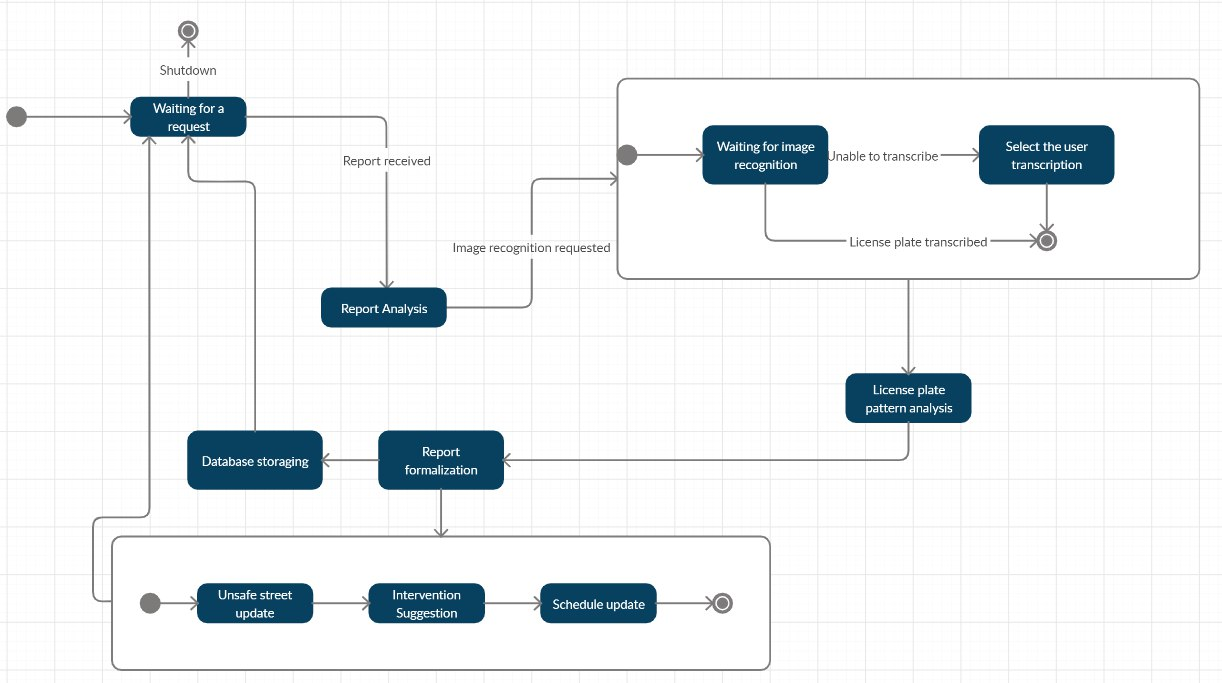
\includegraphics[width=1.0\textwidth]{UML_diagrams/State}
    \caption{Report state diagram}
    \label{fig:state}
\end{figure}
\newpage
  \section{Product Functions}
  \subsection{Send a report}
This is one of the most important function of the service. After the user has successfully registered/logged in to the application, he can choose to send a report of a violation to the officers. This is performed by taking a picture of the car that committed the violation. After the device took the picture the application asks the user to choose from a list of common violations the category that best describes the event (i.e. No parking zone, Double parking). When this information is provided the application gathers some other data in order to have a correct and useful report. In particular it gets: 
\begin{itemize}
  \item The data related to the user who wish to send the report (User ID);
  \item The local time and date gathered from the phone OS;
  \item The information about the street where the user took the picture (Obtained by the GPS coordinates of the user).
\end{itemize}

The user can also optionally add the car plate numbers and the name of the street in case, for example, the application misrecognized the street from the GPS coordinates. When all the necessary data are correctly gathered, the report is sent to the backend system that will handle the request. The user can then consult the history section of the application to monitor the status of its report.

\subsection{Receiving a report - Plate recognition}
The specification document states that the license plate needs to be extracted from the image in order to save it as a correct report. In order to extract the plate number from an image an external service is used. This choice was made because, for this kind of application, an established and robust, high accuracy recognition service will certainly work better than a recognition system that has to be built from scratch only for this kind of purpose. Therefore the backend system runs a task that listens for new reports and as soon as it receives a new one it immediately sends the image contained in the message to the plate recognition service. After the elaboration, the service returns the response of the recognition algorithm that should contain the text transcription of the plate. Note that if for some reason (i.e. bad picture) the plate recognition system can't recognize the plate, the backend system will instead use the plate number inserted by the user if provided; if not provided the violation won't be associated to any plate number. After this recognition step the backend system will interact with the database to create a record that contains the licence plate (if recognized/provided) and all the other information sent in the report. It is important to highlight the fact that the photo won't be discarded after the recognition as they can still be used for legal purposes.

\subsection{Information mining}
The system offers to both users and authorities the possibility to analyse the registered data although the level of visibility differs with respect to the utilizator. 
Users can only see the streets with the highest frequency of violations via the map present in the mobile application. Authorities instead have a wider access to data, that is to say they can access to all registered reports. Via the Web application they can also perform queries on the database (only selection queries) to mine the desired data and compute statistics and metrics for a deeper analysis. The role based approach has been designed in order to guarantee the privacy of car owners with respect to the users of the application. Therefore they will only be allowed to consult for the MDS.

\subsection{Scheduling technicians on violations}
The system offers to LSAs the possibility to manage the violation reports by scheduling them to one or more of their technicians.
Scheduled technicians will have the possibility to change the violation report status (from scheduled) to solved once they patrolled the street and confirmed/rejected the violation.

\subsection{Crossing data with the municipality}
The backend system offers the possibility to interact with an external service, offered by the municipality, that provides data regarding car accidents happened in the municipality area. SafeStreets can define the potential unsafe areas of the municipality by merging car accidents data and violation reports stored by the application. The system can then suggest to the local system administrator possible interventions in order to improve the safety of this areas. It is important to note that the data offered by this service need to be structured in a standard way recognizable by the backend system, otherwise the information crossing will not provide any results.

  \section{User Characteristics}
  \subsection{Actors}

\begin{itemize}
    \item \textit{Visitor}: a person without a SafeStreet account. Visitors can only have access to the homepage and the registration form of the mobile application;
    \item \textit{User/ Mobile user}: a person correctly registered to the SafeStreet account service. Users/Mobile users can perform any of the actions made available by the SafeStreet mobile application; 
    \item \textit{Recognized authority}: a recognized authority (Police station/ municipality) which submitted to SafeStreet and can interact with it through its web application interface;
    \item \textit{Local system administrator/Police corporal}: a person which belongs to a recognized authority, in charge of dealing police technician accounts and scheduling patrols;
    \item \textit{Police technician}: a policeman encharged of dealing with the violations report. He/She patrols the unsafe areas and gives fines to the reported cars in case of violations;
    \item \textit{Third party recognition service}: an image recognition service which allows SafeStreet to extract car plates from the violation report's images.
\end{itemize}


  \section{Constraints}
  \subsection{Regulatory policies}
The user information is stored accordingly to the GDPR policies in order to guarantee the privacy of individuals.
\begin{itemize}
    \item No data is shared with third parties for commercial purposes;
    \item All reported images and violation data are stored safely through encryption methods. The third party system used for image recognition can not store any information/image which identifies;
    \item Any additional information, such as GPS position or Camera access, is promptly asked to the user before performing the specific operation, accordingly to the Android/IOS standards.
\end{itemize}


\subsection{Hardware limitations}
\begin{itemize}
    \item Mobile applications:
    \begin{itemize}
        \item Any kind of modern smartphone;
        \item Internet connectivity;
        \item Camera;
        \item GPS.
    \end{itemize}
    \item Web application:
    \begin{itemize}
        \item Browser (any HTTP client);
        \item Internet connectivity.
    \end{itemize}
\end{itemize}
\subsection{Interface to other applications}
A certified external image recognition service deals with the car plate recognition through report's images.\newline
Report's information are stored in a cloud database which guarantees data encryption and information retrieving through authentication.
  \section{Assumptions and dependencies}
  As far as the specification document is concerned, it is necessary to specify some details and to state clearly a few ambiguous points. In order to better clarify those situations the following assumptions are intoduced.
\subsection{Text Assumptions}
\begin{itemize}
    \item \textbf{Violation report}
        \begin{itemize}
            \item The information sent by user in the violation report includes: the license plate image and an optional textual transcription, its position coordinates (extracted automatically from the smartphone GPS) and the violation metadata;
            \item The suitable metadata descripted in the specification document is intended as a choice of the law infringment and a textual description of the event;
            \item Given the coordinates of the violation, the system is able to retrieve the address from which the report was sent;
            \item Every time a report is received, the system will ask the image recognition service for the license plate textual transcription.
            \item A license plate textual transcription is considered correct if it fits into one of the common standard of the EU states. In case of wrong textual transcription of the license plate from the image recognition service:
            \begin{itemize}
                \item The textual transcription provided by the user is taken into account. After a previous check, the provided license plate will be considered as correct.
                \item If the user has not sent a textual transcription, the violation is not associated to any license plate number;
            \end{itemize} 
        \end{itemize}
    \item \textbf{Mining information} 
        \begin{itemize}
            \item End users are allowed to mine information about the violation reports that they sent. Also, they can have access only to the (map visualization or list) streets with the highest frequency of violation reports (called "most dangerous" streets (MDS) from now on);
            \item Authorities can mine information concerning all the stored information in the SafeStreet system, such as MDS or the list of cars with an high number of violation reports.
        \end{itemize}
    \item \textbf{Suggested intervention}
        \begin{itemize}
            \item Only authorities are allowed to have access to the suggested intervention on unsafe areas identified by the system.
        \end{itemize}
    \end{itemize}
\subsection{Domain assumptions}
\begin{itemize}
    \item {[D1]}  A picture taken with a smartphone is performed with a quality sufficient for the image recognition service to transcribe it;
    \item {[D2]}  The reported picture contains only the license plate of the car that committed the violation and not others;
    \item {[D3]}  The GPS information collected from the smartphone of a user has an accuracy of less than 5 meters;
    \item {[D4]} The timestamp collected from the smartphone is synchronized with the CET standard;
    \item {[D5]} The users can only report violations occured in Europe;
    \item {[D6]} Reports are only sent through a secure connection channel;
    \item {[D7]} The users reports all the violation that they detect;
    \item {[D8]} The users send report containing correct information about the detected violation;
    \item {[D9]} The municipality system stores correctly all the information concerning car accidents;
    \item {[D10]} The municipality legacy system allows SafeStreet to retrieve information about the car accident among a certain area;
    \item {[D11]} The image recognition service is able to detect and transcribe license plates;
\end{itemize}



  

\end{document}
  

